\documentclass[12pt, a4paper]{report}
%\documentclass[11pt, a4paper]{article}

%====================== PACKAGES ======================
\usepackage[french]{babel}

\frenchbsetup{StandardLists=true}
\usepackage{enumitem}
\usepackage{pifont}

\usepackage[utf8x]{inputenc}
%\usepackage[latin1]{inputenc}

%pour gérer les positionnement d'images
\usepackage{float}
\usepackage{amsmath}
\DeclareMathOperator{\dt}{dt}
\usepackage{graphicx}
%\usepackage{tabularx}
\usepackage[colorinlistoftodos]{todonotes}
\usepackage{url}

%pour les informations sur un document compilé en PDF et les liens externes / internes
\usepackage[pdfborder=0]{hyperref}
\hypersetup{
	colorlinks = true
	}

%pour la mise en page des tableaux
\usepackage{array}
\usepackage{tabularx}
\usepackage{multirow}
\usepackage{multicol}
\setlength{\columnsep}{50pt}

%pour utiliser \floatbarrier
%\usepackage{placeins}
%\usepackage{floatrow}

%espacement entre les lignes
\usepackage{setspace}

%modifier la mise en page de l'abstract
\usepackage{abstract}

%police et mise en page (marges) du document
\usepackage[T1]{fontenc}
\usepackage[top=2cm, bottom=2cm, left=2cm, right=2cm]{geometry}

%Pour les galerie d'images
\usepackage{subfig}

\usepackage{pdfpages}

\usepackage{tikz}
\usetikzlibrary{trees}
\usetikzlibrary{decorations.pathmorphing}
\usetikzlibrary{decorations.markings}
\usetikzlibrary{decorations.pathreplacing,calligraphy}
%\usetikzlibrary{decorations}
\usetikzlibrary{angles, quotes}
\usepackage{verbatim}

\usepackage{appendix}

\usepackage{comment}

\usepackage{xcolor}

%\PreviewEnvironment{tikzpicture}
%\setlength\PreviewBorder{0pt}%

%====================== INFORMATION ET REGLES ======================

%rajouter les numérotation pour les \paragraphe et \subparagraphe
\setcounter{secnumdepth}{4}
\setcounter{tocdepth}{4}

\hypersetup{							% Information sur le document
pdfauthor = {Stephan Runigo},			% Auteurs
pdftitle = {Documentation},			% Titre du document
pdfsubject = {Documentation},		% Sujet
pdfkeywords = {Document},	% Mots-clefs
pdfstartview={FitH}}	% ajuste la page à la largeur de l'écran
%pdfcreator = {MikTeX},% Logiciel qui a crée le document
%pdfproducer = {} % Société avec produit le logiciel

%======================== DEBUT DU DOCUMENT ========================
%
\begin{document}
%
%régler l'espacement entre les lignes
\newcommand{\HRule}{\rule{\linewidth}{0.5mm}}
%
% Titre, résumé, ... %
%
%
\begin{titlepage}
%
~\\[1cm]

\begin{center}
%\includegraphics[scale=0.5]{./presentation/chambreABulle}
\end{center}

\textsc{\Large }\\[0.5cm]

% Title \\[0.4cm]
\HRule

\begin{center}
{\huge \bfseries Spiritualisme et\\
matérialisme\\[0.4cm] }
\end{center}

\HRule \\[1.5cm]


\vfill

\hfill
\begin{minipage}{0.4\textwidth}
\begin{flushright} \large
%\emph{Auteur:}\\
%Stephan \textsc{Runigo}
Extraits de dictionnaires et d'encyclopédies
\end{flushright}
\end{minipage}

\vfill
{\sf \footnotesize
\begin{itemize}[leftmargin=1cm, label=\ding{32}, itemsep=1pt]
\item {\bf Objet : } Étudier les concepts liés au spiritualisme et au matérialisme.
\item {\bf Contenu : } Définitions et philosophie encyclopédique.
\item {\bf Public concerné : } Néophyte.
\end{itemize}
}

\vfill

% Bottom of the page
{\large \today}

\end{titlepage}

\newpage
%\begin{center}
\Large
Résumé
\normalsize
\end{center}
\vspace{3cm}
\begin{itemize}[leftmargin=1cm, label=\ding{32}, itemsep=21pt]
\item {\bf Objet : éclairer } .
\item {\bf Contenu : définitions} .
\item {\bf Public concerné : néophyte} .
\end{itemize}

\vspace{3cm}

résumé.

\vspace{3cm}

Ce document contient des définitions provenant de divers dictionnaires.




\thispagestyle{empty}

\begin{center}
\Large
%Introduction
Préambule
\normalsize
\end{center}
\vspace{3cm}

Ce document est une compilation d'articles provenant de quatre ouvrages : un dictionnaire encyclopédique de poche, {\it La pratique de la philosophie} destiné aux lycéens, une encyclopédie de la philosophie destinée aux néophytes, et le dictionnaire philosophique d'André Comte-Sponville.
les chapitres contiennent les articles des trois premiers ouvrages, les articles du dictionnaire de philosophie d'André Comte-Sponville sont reproduits en annexe.

\vspace{1.3cm}

Chaque chapitre contient les articles correspondant à une notion particulière. Ces notions ont été choisies en raison de leurs liens avec la question du hasard. Ces choix ont été guidés : 1. Par les renvois vers d'autres articles présent dans les ouvrages, 2. Mes propres choix, liés à mes connaissances, 3. La volonté d'obtenir une quantité raisonnable d'information.

\vspace{1.3cm}

Dans {\it La pratique de la philosophie}, l'article concernant la nécessité renvoit à des textes de Spinoza dont le choix reste subjectif à l'ouvrage. J'ai néanmoins reproduit en annexe ces textes ainsi que l'article concernant Spinoza. (les autres annexes sont d'autres renvois de cet ouvrage)

Les articles compilés dans ce document comportent donc les choix "discutables" réalisés dans les trois ouvrages utilisés. Il s'agit donc d'un document de "travail" destiné à apporter quelques points de vues philosophiques de manière relativement élémentaire.

\vspace{1.3cm}

Les trois premiers chapitres abordent les thèmes du hasard, de la nécessité puis du vitalisme. Les chapitres suivants élargissent le champ de vision philosophique en abordant les thèmes du déterminisme, de la contingence et de la providence.

\vspace{2.3cm}

\hfill Stephan Runigo

%%%%%%%%%%%%%%%%%%%%%%%%%%%%%%%%%%%%%%%%%%%%%%%%

%
\newpage
%
%

\thispagestyle{empty}
\begin{center}
\Large
%Introduction
Les ouvrages utilisés
\normalsize
\end{center}

\vspace{1.3cm}

Premières de couverture

\begin{center}
\includegraphics[scale=0.43]{./presentation/dictionnaire-1}
\hfill
\includegraphics[scale=0.43]{./presentation/pratique-1}
\hfill
\includegraphics[scale=0.43]{./presentation/encyclopedie-1}
\end{center}

\vspace{1.3cm}

Quatrièmes de couverture

\begin{center}
\includegraphics[scale=0.43]{./presentation/dictionnaire-2}
\hfill
\includegraphics[scale=0.43]{./presentation/pratique-2}
\hfill
\includegraphics[scale=0.43]{./presentation/encyclopedie-2}
\end{center}



%\newpage
%

%
% Table des matières
\tableofcontents
\thispagestyle{empty}
\setcounter{page}{0}
%
%espacement entre les lignes des tableaux
\renewcommand{\arraystretch}{1.5}
%
%====================== INCLUSION DES CHAPITRES ======================
%
~
\thispagestyle{empty}
%recommencer la numérotation des pages à "1"
\setcounter{page}{0}
\newpage
%
\chapter{L'Éthique}
%
%{\footnotesize XIX$^\text{e}$} siècle — {\bf }{\it }{\it «  »}
%https://www.les-philosophes.fr/spinoza/livres-achat/spinoza-ethique.html
%1/10

\section{Livre I : De Dieu}
%%%%%%%%%%%%%%%%%%%%%%%%%%%%%

Dans l’Éthique, Spinoza, fasciné par la rigueur et la clarté du modèle
mathématique, se donne pour visée d’appliquer la {\bf méthode géométrique} à la
philosophie.

On sait que cette méthode procède par définitions, axiomes, puis s’élève de
propositions en propositions rigoureusement {\bf déduites} les unes des autres
jusqu’à atteindre la vérité à démontrer.

\vspace{0.5cm}
Les définitions ont pour objectif d’indiquer précisément le sens des termes
dont on va se servir, afin qu’il n’y ait nulle ambiguïté ou équivoque possible.

Les axiomes posent des vérités considérées comme évidentes, et qui vont servir
de base aux démonstrations. Ce ne sont plus de simples définitions, au sens où
ils ne se contentent pas de déterminer le sens d’un mot dont on va se servir :
ce sont de vrais jugements prédicatifs qui disent quelque chose de quelque
chose et prétendent au statut de vérité évidente.

\vspace{0.5cm}
Prenons quelques exemples de définitions et d’axiomes proposés par Spinoza.

Parmi les définitions, on trouve au livre I, celle, célèbre, de la {\bf cause de soi}
({\it causa sui}) : {\it « Par cause de soi, j’entends ce dont l’essence enveloppe
l’existence, autrement dit ce dont la nature ne peut se concevoir qu’existante »}.

Ou encore celle de la {\bf substance} : {\it « Par substance, j’entends ce qui est en soi
et se conçoit par soi : c’est-à-dire ce dont le concept n’a pas besoin du
concept d’autre chose, d’où il faille le former »}.

Ces deux définitions sont fondamentales, car elles définissent Dieu pour
Spinoza. Dieu est cause de soi, et Dieu est substance. Plus précisément,
Dieu est seule cause de soi, et seule substance.

Parmi les axiomes, on trouve par exemple : {\it « Étant donné une cause déterminée,
il en suit nécessairement un effet, et au contraire, s’il n’y a aucune cause
déterminée, il est impossible qu’un effet s’ensuive »}.

On voit que Spinoza ne se contente pas ici de définir le concept de cause, mais
affirme une vérité reconnue comme évidente sur la réalité du rapport entre un
effet et une cause.

\vspace{0.5cm}
A partir de ce mécanisme argumentatif {\it « more geometrico »}, Spinoza
s’élève donc de propositions en propositions, qu’il déduit les unes des autres.

Par exemple, de la proposition 7 : {\it « A la nature d’une substance appartient
d’exister »}, et de la proposition 8 : {\it « Toute substance est nécessairement
infinie »}, Spinoza déduit la proposition 11 : {\it « Dieu autrement dit une substance
consistant en une infinité d’attributs dont chacun exprime une essence
éternelle et infinie existe nécessairement »}.

\vspace{0.5cm}
Spinoza utilise des termes issus de l’ancienne scolastique : substance,
attribut, essence, etc. Mais il leur donne un sens nouveau, et l’utilisation
de cette méthode géométrique en philosophie est novatrice.

Surtout, les résultats auxquels il va parvenir dans l’Éthique sont éminemment
modernes.

Dieu en effet est certes substance infinie, dont tout le reste n’est
qu’attribut, Dieu certes est perfection, dont tout le reste procède.
Mais Spinoza au livre IV, définit au détour d’une proposition ce qu’il entend
par Dieu : la Nature.

Il parle de la {\it « puissance même de Dieu, autrement dit de la Nature »} :{\it Deus
sive Natura}.

Or si Dieu n’est autre chose que la Nature, il n’y a en fait pas de Dieu. Dieu
n’est qu’un nom donné à la Nature, et il n’y a pas de Dieu transcendant
(extérieur et supérieur) à celle-ci.

C’est donc là un des premiers philosophes qui, au {\footnotesize XVII$^\text{e}$} siècle, développe, de
manière dissimulée pour échapper à la censure, un {\bf athéisme} au cœur de sa
philosophie.

\vspace{0.5cm}
Dieu, autrement dit la Nature, est donc défini comme substance ayant une
infinité d’attributs. Expliquons rapidement le sens traditionnel de ces termes
« substance » et « attribut ». Prenons un homme. Il est riche, grand, célèbre.
Ces déterminations sont des attributs, au sens où elles peuvent être modifiées
sans que le sujet ne disparaisse. Cet homme riche peut devenir pauvre, il
restera tout de même cet individu. Ce sont donc des déterminations non
essentielles d’une personne (ou d’une chose), que l’on appelle des attributs.

%2/10
\vspace{0.5cm}
Les attributs ne sont pas des étants, n’ont pas d’existence consistante en eux
même. En revanche, le sujet porteur de cet attribut (l’homme lui-même) est une
substance. Et ce qu’on ne peut pas lui enlever sans qu’il disparaisse fait
partie de sa substance.

\vspace{0.5cm}
La substance, c’est ce qui se tient en dessous des accidents ({\it sub} : en
dessous, {\it tenere} : se tenir).

Depuis Aristote, ces termes ont ce sens là ; l’homme (substance) a divers
attributs (ou accidents) : beau, grand, naïf, etc. Or Spinoza renverse
radicalement cette perspective. Chez lui, l’homme n’est plus une substance
subsistant en soi.

\vspace{0.5cm}
Il n’est plus en lui-même qu’un {\bf attribut}, un accident, de la seule substance
qui existe véritablement : Dieu, autrement dit la Nature.

Il n’est naturellement pas le seul à être frappé de cette dégradation, de ce
changement ontologique. L’ensemble des étants (tout ce qui est) n’est
qu’attribut de Dieu.

Chez les stoïciens, l’homme n’était certes compris que comme partie du Tout,
qui est le cosmos. Mais l’homme restait substance, parmi les substances.
Ici ce n’est plus le cas.

\vspace{0.5cm}
On comprend dès lors pourquoi Spinoza dit que {\it « tout ce qui est est en Dieu
et rien ne peut sans Dieu ni être ni se concevoir »}.

Dieu est cause de tout, mais pas au sens traditionnel où tout serait un effet
de son intellect et de sa volonté infinie. C’est humaniser Dieu que de lui
accorder ces facultés (intellect et volonté). A la rigueur, on peut le lui
accorder métaphoriquement, mais alors il faut garder à l’esprit que l’un et
l’autre de ces deux attributs représentent réellement en Dieu "toute autre
chose que ce que les hommes, d’ordinaire, entendent vulgairement par là".
La volonté et l’intellect réels de Dieu divergent de notre conception
traditionnelle de la volonté et de l’entendement tout autant que le Chien
zodiacal (la constellation du Chien) diffère de l’animal.

En fait, Dieu est {\bf cause de tout} non pas au sens où il décide de tout, mais au
sens où tout découle nécessairement de sa nature.

\vspace{0.5cm}
Spinoza se place dans une perspective résolument {\bf déterministe}, au sens où pour
lui tout événement, loin de se produire par hasard, découle d’une cause,
elle-même dérivant d’une cause antérieure, qui n’est à son tour que l’effet
d’une cause précédente, etc. En remontant la chaîne des causes, on parvient à
la 1ère des causes qui est la cause de soi (causa sui) : Dieu.

Donc tout être humain, tout étant, tout événement, est un effet nécessaire de
la nature de Dieu, dans son déploiement historique. Rien n’est contingent, rien
ne se produit par hasard : {\it « Dans la nature des choses, il n’y a rien de
contingent, mais tout y est déterminé par la nécessité de la nature divine,
à exister et à opérer d’une manière précise »}.

Néanmoins Spinoza appelle « contingentes » les choses singulières, non pas au
sens où elles se produiraient sans cause, mais au sens où leur cause ne se
situe pas en elle-même, mais dans d’autres causes ou événements ultérieurs.
Seul Dieu n’est pas contingent dans la mesure où en tant que cause de soi,
il porte sa cause en lui-même.

\vspace{0.5cm}
Spinoza peut distinguer alors deux choses : la « nature naturante » : Dieu
lui-même, cette cause de soi d’où tout provient, et la « nature naturée »,
à savoir l’ensemble des attributs créés par ce dynamisme et qui restent en Dieu.

Voici la définition précise de ces deux termes :

Nature naturante : {\it « ce qui est en soi et se conçoit par soi, autrement dit
tels attributs de la substance, qui expriment une essence éternelle et infinie »}.

Nature naturée : {\it « tout ce qui suit de la nécessité de la nature de Dieu, ou
de ses attributs, ou des manières de ses attributs, en tant qu’on les considère
comme des choses qui sont en Dieu »}.

\vspace{0.5cm}
Les étants puisqu’ils découlent de la nature parfaite de Dieu, sont en
eux-mêmes parfaits, ainsi que les événements qui se produisent : {\it « les choses
ont été produites par Dieu avec la suprême perfection : puisque c’est de la
plus parfaite nature qui soit qu’elles ont suivi nécessairement »}.

%3/10
\vspace{0.5cm}
On remarque que certains éléments se rapprochent du stoïcisme (le déterminisme,
la perfection du monde, la nature comme Dieu), et que l’on aurait pu les voir
écrits dans les Pensées de Marc-Aurèle.

Mais ce sont les seuls. La théorie de Spinoza se distingue radicalement du
stoïcisme sur l’ensemble des autres points. Elle a une originalité et une
consistance propre à elle.

\vspace{0.5cm}
Dans le célèbre appendice du livre I, Spinoza insiste sur l’importance qu’il y
a à lutter contre les {\bf préjugés}. Ces préjugés sont les superstitions véhiculées
par la religion, en premier lieu le {\bf finalisme}, c’est-à-dire l’idée que l’homme
est à la fin de la Création (ou encore que Dieu a tout créé pour l’homme, en
vue de son bonheur).

Cela repose sur un autre préjugé, à savoir que l’homme se considère comme
libre, parce qu’il a conscience de vouloir ou de désirer des choses. Mais
il n’est pas conscient du fait qu’il y a des causes qui le déterminent
nécessairement à vouloir ou à désirer ces choses. Ce n’est pas réellement une
volonté libre dont il dispose, il n’est donc {\bf pas libre} : {\it « les hommes se croient
libres, pour la raison qu’ils ont conscience de leurs volitions et de leur
appétit, et que les causes qui les disposent à appéter et à vouloir, ils les
ignorent, et n’y pensent pas même en rêve »}.

L’idée selon laquelle les Dieux ont tout créé pour les hommes, pour que ces
derniers les honorent, et que plus on les honore, plus on en tirera de grands
bénéfices (dont celui de la vie éternelle), relève de la superstition. On
comprend pourquoi Spinoza a été excommunié par ses coreligionnaires juifs
d’Amsterdam, et ce même si l’Éthique n’est jamais parue de son vivant.

\vspace{0.5cm}
En réalité pour Spinoza, c’est le finalisme (à l’œuvre dans le
judéo-christianisme) qui est impie : {\it « cette doctrine supprime la perfection
de Dieu : car si Dieu agit à cause d’une fin, c’est nécessairement qu’il aspire
à quelque chose qui lui manque »}.

Or puisque les hommes pensent que les choses sont faites pour eux, ils ont
forgé les notions (ou fictions) suivantes : {\it « le bien, le mal, l’ordre, la
confusion, le chaud, le froid, la beauté et la laideur »} et puisqu’ils pensent
être libres {\it « la louange et le blâme, le péché et le mérite »}.

En réalité, rien de tout cela n’existe. Cela n’a de sens que par rapport à
nous, mais ne renvoie à aucune réalité en soi. Il n’y a pas de bonnes ou de
mauvaises actions, il n’y a que des actions qui se déroulent nécessairement,
découlant de la substance divine infinie, dont certaines nous arrangent et
d’autres nous nuisent.

De même, les hommes appellent « ordre » ce qui leur est facile d’imaginer,
{\it « comme si l’ordre était quelque chose dans la nature indépendamment de notre
imagination »}.

Un dernier exemple : {\it « si le mouvement que reçoivent les nerfs à partir des
objets qui se représentent par les yeux contribue à la santé, les objets qui
le causent sont dits beaux, et ceux qui excitent un mouvement contraire laids »}.

Pour résumer : {\it « chacun a jugé des choses d’après la disposition de son cerveau
et a pris pour les choses les affections de son imagination »}.

\vspace{0.5cm}
De ce fait, le monde est {\bf parfait}, et ce n’est pas parce que certaines choses
ou événements nuisent aux hommes qu’il en perd sa perfection.


%
%{\footnotesize XIX$^\text{e}$} siècle — {\it }{\it «  »}{\bf }
%https://www.les-philosophes.fr/spinoza/livres-achat/spinoza-ethique.html

\section{Livre II : de l’Esprit}
%%%%%%%%%%%%%%%%%%%%%%%%%%%%%%%%%%%%%%%%%%

Ici encore, Spinoza commence par poser des définitions et des axiomes.

On relèvera la définition spinoziste du {\bf corps} : {\it « par corps, j’entends une
manière qui exprime, de manière précise et déterminée, l’essence de Dieu en
tant qu’on la considère comme chose étendue »}.

Elle s’inspire de la définition cartésienne du corps comme chose étendue que
l’on trouve dans les Méditations Métaphysiques, qui s’oppose à l’esprit
considéré comme chose pensante. Néanmoins chez Spinoza, ces deux attributs
caractérisent Dieu, ou la nature : {\it « la Pensée est un attribut de Dieu,
autrement dit Dieu est chose pensante »} et {\it « l’étendue est un attribut de Dieu,
autrement dit Dieu est chose étendue »}.

%4/10
\vspace{0.5cm}
Si l’homme pense, il n’est pas une substance mais {\it « l’essence de l’homme est
constituée par des modifications précises des attributs de Dieu »}, {\it « quelque
chose qui est en Dieu, et qui sans Dieu ne peut ni être ni se concevoir,
autrement dit une affection qui exprime la nature de Dieu de manière précise
et déterminée »}.

On voit donc que Spinoza se distingue fondamentalement de Descartes sur ce
point, pour qui l’homme est formé de deux substances, la substance pensante
et la substance étendue.

\vspace{0.5cm}
Pour Spinoza, l’esprit humain n’est pas une substance, mais {\it « une partie de
l’intellect infini de Dieu »}. Ce qui permet cette belle affirmation : {\it « Dieu
constitue la nature de l’Esprit humain »}.

Le corps quant à lui est {\it « l’objet de l’idée constituant l’esprit humain »} ou
encore {\it « une manière de l’Etendue précise et existant en acte, et rien d’autre »}.

\vspace{0.5cm}
Cette conception permet de donner une solution au problème de {\bf l’union du corps
et de l’esprit} fondamentalement différente de celle de Descartes.

Tout d’abord, il y a bien union : {\it « Que l’Esprit est uni au Corps, nous l’avons
montré de ce que le Corps est objet de l’Esprit »}.

Ensuite il n’y a pas deux choses distinctes, mais une seule et même chose,
envisagée sous {\bf deux points de vue différents} : {\it « l’idée du Corps et le Corps,
c’est-à-dire l’Esprit et le Corps, est un seul et même individu, que l’on
conçoit tantôt sous l’attribut de la Pensée, tantôt sous celui de l’Etendue »}.

\vspace{0.5cm}
Cette solution résolument novatrice du problème de l’esprit et corps amène
Spinoza à reconsidérer la nature de deux facultés : la connaissance et la
volonté. Ces deux facultés sollicitent en effet, dans leur acception
traditionnelle, le corps et l’esprit.

Les philosophes ont en effet essayé de déterminer l’importance du corps dans
le processus de la connaissance. Comment connaît-on une chose ? Au moins dans
un premier temps grâce à la perception du corps.

Pour Spinoza, nous percevons par les sens les choses extérieures, et nous en
formons des concepts universels. Mais les sens nous les présentent {\it « de manière
mutilée et confuse, et sans ordre pour l’intellect »}. Ce pourquoi ce premier
genre de connaissance est imparfait : {\it « j’ai l’habitude d’appeler de telles
perceptions connaissance par expérience vague »}.

Cette connaissance du {1$^\text{er}$} genre regroupe ce qu’on l’on entend par opinion ou
imagination.

Elle est l’unique source de fausseté.

\vspace{0.5cm}
La connaissance du {2$^\text{nd}$} genre désigne la raison, c’est-à-dire le fait
d’atteindre les notions communes et les idées adéquates des propriétés
des choses.

La connaissance du {3$^\text{ème}$} genre est une science intuitive, qui {\it « procède de
l’idée adéquate de l’essence formelle de certains attributs de Dieu vers
la connaissance adéquate de l’essence des choses »}.

Ces deux derniers genres de connaissance sont nécessairement vrais.

\vspace{0.5cm}
La vérité d’une idée apparaît dans son évidence : {\it « qui a une idée vraie, en
même temps sait qu’il a une idée vraie, et ne peut pas douter de la vérité
de la chose »}.

Puisque notre esprit est {\it « une partie de l’intellect infini de Dieu »}, {\it « il est
tout aussi nécessaire que les idées claires et distinctes de l’esprit soient
vraies, que cela est nécessaire des idées de Dieu »}.

{\bf La raison} perçoit les choses telles qu’elles sont en soi. Elle saisit donc
leur caractère nécessaire ; de même {\it « il est de la nature de la raison de
percevoir les choses sous une certaine espèce d’éternité »} ({\it sub specie
aeternitatis}).

\vspace{0.5cm}
Spinoza doit également, suite à sa nouvelle conception de l’union de l’esprit
et du corps, revisiter la notion traditionnellement admise de {\bf volonté}. En
effet la volonté est classiquement une faculté par laquelle l’esprit agit sur
le corps. Mais qu’est la volonté, si corps et esprit sont une même chose,
envisagée sous deux angles différents ?

%5/10
\vspace{0.5cm}
Spinoza commence par rappeler qu’en fonction de sa conception déterministe,
{\it « dans l’Esprit nulle volonté n’est absolue, autrement dit libre, mais l’Esprit
est déterminé à vouloir ceci ou cela par une cause, qui elle aussi est
déterminée par une autre, et celle-ci à son tour par une autre, et ainsi à
l’infini »}.

Cela vaut de la même manière pour les prétendues facultés de comprendre, de
désirer, d’aimer... qui sont donc {\it « soit purement fictives, soit rien que des
étants métaphysiques, autrement dit des universaux que nous avons coutume de
former à partir des particuliers »}.

\vspace{0.5cm}
En fait, ce qui est réel, c’est non pas la volonté mais telle ou telle {\bf volition}
particulière qui accompagne telle ou telle de nos idées : {\it « l’intellect et la
volonté ont avec telle idée ou volition le même rapport que la pierrité avec
telle pierre, ou que l’homme avec Pierre et Paul »}.

Il faut remarquer que Spinoza n’entend pas par volonté le désir (duquel il
traitera dans le livre suivant), mais {\it « la faculté d’affirmer et de nier la
vérité ou la fausseté de quelque chose »}.

\vspace{0.5cm}
De plus les volitions elles-mêmes disparaissent, puisque l’idée enveloppe en
elle-même sa propre négation ou affirmation (ce en quoi elles ne sont pas des
simples images, ou peintures, à laquelle l’esprit décide ou non de donner son
assentiment). Elles portent en elles-mêmes leur propre assentiment.

Prenons un exemple : ce n’est pas la volonté qui refuse l’idée de se jeter dans
le vide, c’est cette idée elle-même qui porte son propre principe de persuasion
(ou de refus). De même que la vérité se manifeste d’elle-même, de par sa propre
lumière ou évidence, comme on l’a vu.

Ce pourquoi Spinoza peut affirmer {\it « dans l’esprit il n’y a aucune volition,
autrement dit aucune affirmation et négation, à part celle qu’enveloppe l’idée,
en tant qu’elle est idée »}.

Il n’y a donc, de ce fait, aucune différence entre volonté et intellect.
Comprendre une idée, c’est y adhérer ou la refuser, selon l’affirmation ou la
négation qu’elle porte. Ou encore, c’est l’idée elle-même qui s’impose à nous,
ou au contraire, suscite en nous une opposition.

\vspace{0.5cm}
Pourtant, certains n’adhèrent-ils sincèrement pas à des idées fausses ? Spinoza
le nie : ils ne sont pas certains de cette idée, au mieux, ils ne doutent pas.
Or la certitude est quelque chose de positif et non une simple privation de
doute. Seule une idée vraie peut provoquer la certitude.

De la même manière, Spinoza balaie d’autres objections. Par exemple, le fait
que depuis Descartes, on distingue la volonté de l’intellect car la première
est infinie, tandis que le second est fini. Ou encore qu’alors on ne pourra
choisir entre deux idées ayant la même force d’assentiment, tel {\bf l’âne de
Buridan} qui se laisse mourir parce qu’il est placé à égale distance de foin
et d’eau.

Spinoza commence à envisager les conséquences pratiques des deux premiers
livres. La doctrine spinoziste permet de rendre {\it « l’âme tranquille de toutes
les manières »}, du fait qu’ {\it « elle enseigne que nous agissons par le seul
commandement de Dieu, et que nous participons de la nature divine »} et enfin
que {\it « notre suprême félicité consiste dans la seule connaissance de Dieu »}.


%
%{\footnotesize XIX$^\text{e}$} siècle — {\it }{\it «  »}{\bf }
%https://www.les-philosophes.fr/spinoza/livres-achat/spinoza-ethique.html

\section{Livre III : des affects}
%%%%%%%%%%%%%%%%%%%%%%%%%%%%%%%%%%%%

Les affects désignent les passions et désirs humains. Ce serait une erreur de
considérer qu’ils sont {\bf contre-nature}. Au contraire puisque tout procède
nécessairement de la substance divine, tout est naturel : {\it « pour la plupart,
ceux qui ont écrit des affects semblent traiter, non de choses naturelles qui
suivent les lois communes de la nature, mais de choses qui sont hors de la
nature. On dirait même qu’ils conçoivent l’homme dans la nature comme un
empire dans un empire. Car ils croient que l’homme perturbe l’ordre de la
nature plutôt qu’il ne le suit »}.

C’est là une profonde erreur, au contraire {\it « rien ne se fait dans la nature
que l’on puisse attribuer à un vice de celle-ci ; car la nature est toujours
la même, et a partout une seule et même vertu et puissance d’agir »}.

%6/10
\vspace{0.5cm}
De ce fait, les affects apparaissent ou disparaissent selon la même nécessité
que les choses ou événements. Une science des affects est donc possible : {\it « je
considèrerai les actions et appétits humains comme s’il était question de
lignes, de plans ou de corps »}.

Des définitions qui ouvrent le livre III, nous retiendrons celle des affects :
{\it « par affect, j’entends les affections du corps qui augmentent ou diminuent la
puissance d’agir de ce corps et en même temps les idées de ces affections »}.

\vspace{0.5cm}
La première proposition défend l’idée que notre esprit agit en tant qu’il a des
idées adéquates et pâtit en tant qu’il a des idées inadéquates ; une idée
adéquate étant, selon la définition qu’il en a donnée dans le livre II, une
{\it « idée qui en soi, sans rapport à l’objet, a les propriétés ou les dénominations
intrinsèques de l’idée vraie »}.

Peut-on dire simplement qu’une idée adéquate est une idée vraie ? Probablement,
bien que la formulation de Spinoza laisse plutôt penser qu’une idée adéquate
est une idée bien formée, ayant la forme ou les propriétés d’une idée vraie.

Le corollaire de cette première proposition est remarquable : {\it « l’Esprit est
sujet à d’autant plus de passions qu’il a plus d’idées inadéquates, et au
contraire, agit d’autant plus qu’il a plus d’idées adéquates »}. Peut-on en
déduire qu’un esprit qui atteindrait les dernières vérités serait pure action ?

\vspace{0.5cm}
On a vu dans le livre II la critique spinoziste de la faculté de volonté, et
l’affirmation de l’idée selon laquelle le corps et l’esprit ne sont qu’une
seule et même chose, envisagée selon deux points de vue différents.

C’est pourquoi Spinoza rappelle que {\it « le corps ne peut déterminer l’esprit à
penser, ni l’esprit déterminer le corps au mouvement, ni au repos, ni à quelque
chose d’autre »}.

Ce qui détermine tel ou tel mouvement de notre corps, c’est plutôt un mouvement
antérieur d’un autre corps, ou encore Dieu comme substance étendue ; de même
une pensée ne peut avoir pour cause qu’une autre pensée antérieure, ou Dieu
comme substance pensante.

\vspace{0.5cm}
De ce fait, {\it « l’ordre ou l’enchaînement des choses est un, qu’on conçoive la
nature sous l’un ou l’autre de ces attributs »} autrement dit {\it « l’ordre des
actions et passions de notre corps va par nature de pair avec l’ordre des
actions et passions de notre esprit »}.

Il est donc faux de croire comme on le fait communément que le corps se meut
sous l’impulsion de l’esprit. D’ailleurs, le corps peut se mouvoir sans esprit,
ainsi que le montre l’exemple des somnambules. Enfin, nul ne sait ce que peut
le corps : {\it « l’expérience n’a appris à personne jusqu’à présent ce que le Corps
peut faire par les seules lois de la nature »}.

On croit que le corps est inerte sans esprit ? Spinoza fait remarquer par
l’exemple du sommeil que si le corps est inerte, l’esprit est inerte.

\vspace{0.5cm}
Spinoza développe à nouveau une critique de la volonté, ou du {\bf libre arbitre},
inconciliable avec le déterminisme fondamental de sa pensée : {\it « Ainsi croit le
bébé aspirer librement au lait, et l’enfant en colère vouloir la vengeance, et
le peureux la fuite. L’homme ivre croit que c’est par un libre décret de
l’Esprit qu’il dit ce que, redevenu sobre, il voudrait avoir tu ; alors
pourtant qu’il n’a pas pu contenir l’impulsion qu’il a eu à parler »}.

Pour synthétiser : {\it « les hommes se croient libres, pour la seule raison qu’ils
sont conscients de leurs actions et ignorants des causes par quoi elles sont
déterminées »}.

\vspace{0.5cm}
La célèbre proposition 6 affirme le principe du {\bf conatus} : {\it « chaque chose, autant
qu’il est en elle, s’efforce de persévérer dans son être »}.

Toute chose en effet s’oppose à ce qui pourrait venir supprimer son existence.
Or cet effort, cette tendance fondamentale en tout être, n’est rien d’autre que
la volonté (lorsqu’on le considère du point de vue de l’esprit), ou le désir,
(lorsqu’on le considère à la fois du point de vue de l’esprit et du corps).

%7/10
\vspace{0.5cm}
Spinoza utilise indistinctement les termes « appétit » ou « désir » mais fait
cette précision terminologique : le désir est un appétit dont l’homme est
{\bf conscient} : {\it « le Désir est l’appétit avec la conscience de l’appétit »}.

Cet effort, autrement dit, le désir, est si fondamental qu’il {\it « n’est rien
d’autre que l’essence même de l’homme »}.

Si nous désirons ou voulons une chose, c’est n’est pas parce que nous la
jugeons bonne ; {\it « au contraire, si nous jugeons qu’une chose est bonne, c’est
précisément parce que nous nous y efforçons, nous la voulons, ou aspirons à
elle, ou la désirons »}.

\vspace{0.5cm}
L’esprit peut pâtir de grands changements et passer à une perfection tantôt
moindre, tantôt plus grande. C’est ici que l’on trouve la célèbre définition
de la {\bf joie} spinoziste : {\it « par Joie, j’entendrai donc une passion par laquelle
l’Esprit passe à une plus grande perfection »} ; la tristesse désigne l’affect
contraire.

Les trois affects primaires sont pour Spinoza l’allégresse, la douleur, et le
désir (les deux premiers représentent la joie et la tristesse, mais rapportés
à la fois à l’esprit et au corps).

De la définition spinoziste de la joie se déduit celle de l’amour : {\it « l’Amour
n’est rien d’autre qu’une Joie qu’accompagne l’idée d’une cause extérieure, et
la Haine, rien d’autre qu’une Tristesse qu’accompagne l’idée d’une cause
extérieure »}.

\vspace{0.5cm}
Spinoza définit un grand nombre d’affects, qui naissent de la composition des
trois affects primitifs : l’espérance, la crainte, le désespoir, l’émulation,
etc. et propose un certain nombre de lois psychologiques. Par exemple : {\it « si
nous imaginons que quelqu’un aime ou désire ou a en haine quelque chose que
nous aimons, désirons, ou avons en haine, par là même, nous aimerons, etc.
la chose avec plus de constance »}.

L’auteur de l’Éthique propose pour conclure une définition générale des affects
dans laquelle il répète que {\it « le Désir est l’essence même de l’homme, en tant
qu’on la conçoit comme déterminée, par suite d’une quelconque affection
d’elle-même à faire quelque chose »}, désir étant entendu au sens le plus large,
incluant appétits et volontés.



%
%{\footnotesize XIX$^\text{e}$} siècle — {\it }{\it «  »}{\bf }
%https://www.les-philosophes.fr/spinoza/livres-achat/spinoza-ethique.html

\section{Livre IV : de la servitude humaine ou : des forces des affects}
%%%%%%%%%%%%%%%%%%%%%%%%%%%%%%%%%%%%%%%%%%%%%%%%%%%%%%%%%%%%%%%%%%%%%%%%%

La servitude désigne l’impuissance de l’homme à maîtriser ou contrarier les
affects. Spinoza consacre ce livre à l’étude de ce phénomène, ainsi qu’à
l’étude de ce qu’ont les affects de bien et de mal.

Spinoza commence par examiner l’origine de la formation en nous des concepts
de perfection, de bien et de mal.

Le concept de {\bf perfection} naît du fait de vouloir réaliser quelque chose et
d’atteindre ce but. C’est toujours par rapport à un but que l’on détermine la
perfection de quelque chose : {\it « par exemple si quelqu’un a vu quelque chose
d’inachevé et a su que le but de l’Auteur de cette œuvre était de construire
une maison, il dira que la maison est imparfaite, et parfaite au contraire
sitôt qu’il verra l’œuvre parvenue à la fin que son Auteur avait décidé de
lui donner »}.

En revanche si on ignore le but de l’auteur de l’œuvre, on ne saura si elle
est parfaite ou non.

\vspace{0.5cm}
Puis les hommes forgent des concepts universels, par exemple ceux de tours,
de maisons, etc. et {\it « chacun appela parfait ce qu’il voyait convenir avec
l’idée universelle de la chose »}, {\it « idées qu’ils tiennent pour les modèles des
choses »}. Ils pensent que la nature elle-même les a en vue et se les propose
pour modèles. Si la chose ne convient pas au concept modèle, {\it « ils croient
alors que la nature elle-même a fait défaut ou a péché »}.

Or Spinoza a montré dans l’appendice du livre I que la nature n’agit pas à
cause d’une fin, que le {\bf finalisme} est un préjugé, et que le déterminisme à
l’œuvre dans la nature consacre bien la relation de cause à effet, mais pas
la notion de cause finale.

%8/10
\vspace{0.5cm}
Il est faux donc de croire que la nature soit parfaite ou imparfaite
puisqu’elle ne vise pas un but ; les notions de perfection et d’imperfection
ne sont que des fictions introduites par les hommes.

De même bien et mal {\it « ne désignent pas non plus rien de positif dans les choses,
mais rien d’autre que des manières de penser ou notions que nous formons de ce
que nous comparons les choses entre elles »}.

\vspace{0.5cm}
Pourtant, il faut conserver ces termes, pour pouvoir former une idée de la
nature humaine.

Ce pourquoi Spinoza commence le livre IV en définissant ainsi les concepts
moraux : {\it « par bien et mal, j’entendrai ce que nous savons avec certitude
être un moyen d’approcher ou de s’éloigner du modèle de la nature humaine
que nous nous proposons »}.

De ce fait, la notion de bien ne recouvre d’autre signification que celle
d’{\bf utilité} : {\it « par bien, j’entendrai ce que nous savons avec certitude nous
être utile »}, ou encore de ce qui nous est bénéfique : {\it « nous appelons bien
ou mal ce qui sert ou bien nuit à la conservation de notre être »}.

Enfin, Spinoza rapproche les notions de bien et de mal de celles de joie et
de tristesse, telles qu’il les a défini au livre précédent, comme passage à
une perfection plus ou moins grande : {\it « la connaissance du bien et du mal
n’est rien d’autre que l’affect de joie ou de tristesse, en tant que nous en
sommes conscients »}.

\vspace{0.5cm}
Notons que c’est dans la proposition 4 de ce livre que l’on trouve la célèbre
assimilation de Dieu à la nature : [...] {\it « la puissance même de Dieu, autrement
dit de la Nature »} ({\it Deus sive natura}).

\vspace{0.5cm}
Ce qui fait la servitude humaine, c’est que nous ne pouvons, en vertu du
déterminisme, maîtriser un affect, ou y échapper, de par notre volonté.
En fait, {\it « un affect ne peut être contrarié ou supprimé que par un affect
contraire et plus fort que l’affect à contrarier »}.

Spinoza consacre plusieurs propositions d’ordre psychologiques à préciser
la manière dont un affect s’empare de nous. Par exemple : {\it « un affect par
rapport à une chose que nous imaginons comme nécessaire est toutes choses
égales d’ailleurs, plus intense qu’à l’égard d’une chose possible ou
contingente, autrement dit non nécessaire »}.

\vspace{0.5cm}
Spinoza annonce à partir de la proposition 18, qu’il va maintenant montrer
ce que la raison prescrit, à savoir {\it « quels sont les affects qui conviennent
avec les règles de la raison humaine et quels sont au contraire ceux qui leur
sont contraires »}.

Or {\it « la raison ne demande rien contre la nature, c’est donc elle-même qui
demande que chacun s’aime lui-même, recherche ce qui lui est utile, et
aspire à tout ce qui augmente notre perfection, et que chacun s’efforce
autant qu’il est en lui de conserver son être »}.

Spinoza appelle {\bf vertu} le fait d’ {\it « agir d’après les propres lois de sa nature »},
et donc {\it « le fondement de la vertu est l’effort même pour conserver son être
propre »}.

Ce qui nous est le plus utile, c’est ce qui est de même nature que nous. Donc
{\it « à l’homme rien de plus utile que l’homme »}. De ce fait, l’homme que gouverne
la raison, c’est-à-dire celui qui recherche son propre bonheur, n’aspire à
rien d’autre qu’au bonheur général de tous les hommes.

Spinoza remet donc en cause le principe selon lequel agir vertueusement est
agir de manière désintéressée. L’égoïsme, bien compris, est le fondement de
l’altruisme, pourrait-on dire, puisque autrui nous est foncièrement utile.

\vspace{0.5cm}
Si tous les hommes vivaient sous la conduite de la raison, chacun agirait
selon le souverain droit de nature, c’est-à-dire ferait tout ce qui suit de
la nécessité de sa nature ; mais à cause des affects, qui surpassent la
puissance ou vertu de l’homme, {\it « ils se trouvent entraînés diversement,
contraires les uns aux autres »}.

\vspace{0.5cm}
%9/10
Une solution est que les hommes renoncent à leur droit naturel et s’assurent
mutuellement de ne pas se nuire, en entrant en société.

Puisqu’en effet un affect ne peut être contrarié que par un affect plus fort,
on résistera à un affect (désir de voler quelqu’un) par un autre affect (la
crainte d’un dommage plus grand, à savoir celui d’une punition par la société).

\vspace{0.5cm}
Rappelons que ce livre IV est consacré à l’exposé des raisons de la servitude
humaine, l’homme étant assujetti à la puissance des affects. Or dès ce livre
IV, Spinoza présente les moyens par lesquels l’homme peut conquérir sa liberté,
en luttant contre la puissance des affects.

Il suffit d’utiliser cette puissance même des affects en tournant celle des uns
contre celle des autres, afin qu’ils se {\bf neutralisent}.

\vspace{0.5cm}
Spinoza présente un second moyen de se libérer : {\it « à toutes les actions
auxquelles nous détermine un affect qui est une passion, nous pouvons être
déterminés sans lui par la raison »}.

Notre raison peut créer en nous certains désirs, et ceux-ci, en tant qu’ils
procèdent de la raison nous détermineront à faire ce qui est le mieux pour
nous, autrement dit {\it « ce qui se conçoit adéquatement par la seule essence de
l’homme »}. En effet, {\it « un Désir qui naît de la raison ne peut être excessif »}.

Nous pouvons donc nous libérer des affects, en en créant d’autres {\bf plus adaptés}
ou plus utiles, par {\bf la raison}.

\vspace{0.5cm}
La peur ne fait pas partie des affects raisonnables : {\it « qui est mené par la
crainte, et fait le bien pour éviter le mal, n’est pas mené par la raison »}.

Agir par la raison est agir par joie ou désir. Ce sont les superstitieux qui
cherchent à contenir le mal par la peur de la mort. Ainsi, le sage est celui
qui a dépassé cette peur de la mort, et qui n’y accorde même aucune pensée :
{\it « l’homme libre ne pense rien moins qu’à la mort, et sa sagesse est une
méditation non de la mort, mais de la vie »}.

Enfin, il s’agit de supporter d’une âme égale ce qui nous arrive, y compris
les événements tristes, que nous n’avons pas pu éviter du fait de notre
puissance limitée : {\it « la puissance de l’homme est extrêmement limitée et
infiniment surpassée par la puissance des causes extérieures »}. On peut
rapprocher ce dernier point (subir, se résigner, sans passion négative –
tristesse, peur, envie...) du stoïcisme.



%
%{\footnotesize XIX$^\text{e}$} siècle — {\it }{\it «  »}{\bf }
%https://www.les-philosophes.fr/spinoza/livres-achat/spinoza-ethique.html


\section{Livre V : de la puissance de l’intellect, autrement dit, de la liberté
humaine}
%%%%%%%%%%%%%%%%%%%%%%%%%%%%%%%%%%%%%%%%%%%%%%%%%%%%%%%%%%%%%%%%%%%%%%%%%%%%%%%

Ce livre se consacre {\it « à l’autre partie de l’Éthique, qui porte sur la
manière ou voie qui mène à la liberté »}.

\vspace{0.5cm}
Spinoza a montré la puissance des affects : à la différence de ce que pensaient
les stoïciens, on n’a pas sur nos affects {\it « un empire absolu »}.

Spinoza critique la théorie cartésienne de la glande pinéale et des esprits
animaux, telle que Descartes la développe dans les Passions de l’âme. Ce n’est
donc pas dans le libre-arbitre cartésien que se situe la réelle liberté de l’homme.

C’est ailleurs qu’il faut chercher la manière dont on peut se libérer, de la
puissance des affects.

\vspace{0.5cm}
Tout d’abord, un affect est toujours lié à l’idée d’une cause extérieure. Si
donc on parvient à {\bf supprimer} en soi l’{\bf idée} de cette {\bf cause extérieure}, nous
sommes libérés de l’affect en question : {\it « si nous éloignons une émotion de
l’âme, autrement dit un affect de la pensée d’une cause extérieure, et la
joignons à d’autres pensées, alors l’Amour ou la Haine à l’égard de la cause
extérieure, ainsi que les flottements de l’âme qui naissent de ces affects
seront détruits »}.

Puisque l’amour ou la haine viennent de la joie ou de la tristesse
qu’accompagne l’idée d’une cause extérieure, il suffit de ne plus penser à
cette cause extérieure (l’être aimé d’un amour déçu ou une personne que
l’on déteste) pour que ces passions négatives ne nous affectent plus.

\vspace{0.5cm}
%10/10
D’autre part, il suffit de se former une idée claire et distincte de l’objet
d’une de nos passions pour qu’il cesse d’être une passion : {\it « un affect qui est
une passion est une idée confuse »}.

Pour prendre un exemple simple, sinon simpliste : supposons que je me meure
d’amour pour une personne inaccessible ; il suffit de se former une idée réelle
de l’être aimé pour que je cesse de la désirer, en tout cas si intensément.
Ou encore : il suffit que je prenne conscience de mon amour (et que je cesse
de le subir inconsciemment) pour que celui-ci disparaisse : {\it « un affect est
d’autant plus en notre pouvoir, et l’esprit en pâtit d’autant moins qu’il est
plus connu de nous »}.

\vspace{0.5cm}
C’est de la {\bf connaissance} que provient par conséquent la {\bf liberté} : {\it « telle est
donc la chose à quoi il faut avant tout s’appliquer, à connaître clairement et
distinctement, autant que faire se peut, chacun de nos affects »}.

C’est en effet un seul et même désir qui amène l’homme à agir ou pâtir, selon
qu’il procède d’une idée adéquate ou inadéquate. Formons des idées adéquates
de tous nos désirs, et nous n’en pâtirons plus, mais nous serons acteur de nos
désirs.

Cela est fondamental, car pour Spinoza, ainsi qu’il le montre dans la
proposition 40 : {\it « plus chaque chose a de perfection, plus elle agit et moins
elle pâtit, et inversement »}.

Celui qui parvient à la connaissance parvient à la liberté, mais également à
l’amour : {\it « qui se comprend clairement et distinctement soi-même aime Dieu, et
d’autant plus qu’il se comprend plus soi-même, ainsi que ses affects »}.

\vspace{0.5cm}
Dieu est pour sa part exempt de joie et de tristesse (car il ne peut passer à
une plus ou moins grande perfection), et par suite d’amour ou de haine : {\it « Dieu
à proprement parler n’aime personne et ne hait personne »}.

Pour comprendre Dieu, il faut comprendre les choses singulières. Mais si l’on
atteint Dieu par le {\bf 3$^\text{ème}$ mode de connaissance}, tel qu’il a été défini
antérieurement, c’est-à-dire par la raison, du point de vue de l’éternité,
{\it « l’amour qui en naît est également nécessairement éternel »}.

C’est ce troisième genre de connaissance qui permet donc d’atteindre le
{\bf bonheur} et la liberté complète.

Spinoza attribue tout de même à Dieu un amour intellectuel infini de lui-même,
semblant contredire ce qui précède. Or {\it « l’amour intellectuel de l’esprit envers
Dieu est une partie de l’Amour infini dont Dieu s’aime lui-même »}.

L’esprit humain n’est pas détruit en même temps que le corps, il en reste
quelque chose, la part éternelle de l’Esprit : l’intellect, marque de notre
perfection parce que c’est par lui que nous agissons. Ce qui périt est
l’imagination, {\it « par laquelle seule nous sommes dits pâtir »}.

Le bonheur n’est pas la récompense de la vertu, c’est la vertu même : {\it « ce n’est
pas parce que nous contrarions les plaisirs lubriques que nous jouissons de la
[{\it béatitude}] ; mais au contraire c’est parce que nous jouissons d’elle que nous
pouvons contrarier les plaisirs lubriques »}.

Pour synthétiser : {\it « la béatitude consiste dans l’Amour envers Dieu, qui naît du
3ème genre de connaissance, et qui se rapporte à l’Esprit en tant qu’il agit »}.

Spinoza conclut l’Éthique en distinguant le {\bf sage} de l’{\bf ignorant} : {\it « D’où il
appert combien le Sage est fort et vaut mieux que l’ignorant, qui agit par le
seul appétit lubrique. L’ignorant en effet, outre que les causes extérieures
l’agitent de bien des manières, et que jamais il ne possède la vraie
satisfaction de l’âme, vit en outre presque inconscient et de soi, et de Dieu,
et des choses, et dès qu’il cesse de pâtir, aussitôt il cesse aussi d’être »}.
Tandis que le Sage {\it « conscient de soi, et de Dieu, et des choses avec une
certaine nécessité éternelle, jamais il ne cesse d’être »}.


\vfill

\begin{center}
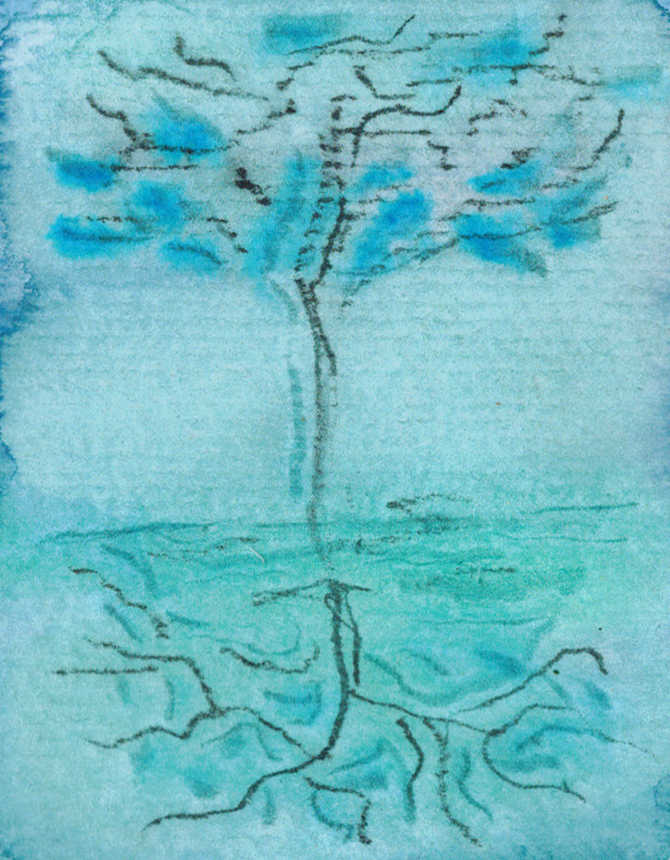
\includegraphics[scale=1.8]{./ethique/arbre}
\end{center}

\vfill


%

%
%\input{./chapitre2/chapitre2.tex}
%
%====================== INCLUSION DE LA BIBLIOGRAPHIE ======================
%
%récupérer les citation avec "/footnotemark" : 
\nocite{*}
%
% choix du style de la biblio
\bibliographystyle{plain}
%
% inclusion de la biblio
\cleardoublepage
\addcontentsline{toc}{chapter}{Bibliographie}
\bibliography{bibliographie.bib}
%
%====================== FIN DU DOCUMENT ======================
%
\end{document}
%%%%%%%%%%%%%%%%%%%%%%%%%%%%%%%%%%%%%%%%%%%%%%%%%%%%%%%%%%%%%%%%%%%%%%%%%%%%%%%%%
